\section{Testmetode}
\label{sec:metode}
\subsection{Måling av tapsledd}
\label{sec:metode-tap}
\label{sec:ml-serien}
\label{sec:utsnurring-behandling}
Energien i svinghjulet går tapt til sluring ved nedsetting, friksjon i lagrene på svinghjulsakselen og hjulakslene, tap i tannhjulsinngrepet og rullemotstand mellom dekk og underlag. Simuleringen trenger en verdi for hvert av dem (tabell~\ref{tab:sim-parametre}).

\paragraph{Lagrene på svinghjulsakselen} er målt med utsnurring. Bilen holdes løftet, svinghjulet trekkes opp med snor, og en Hall-sensor registrerer to magneter på akselen (figur~\ref{fig:esp-oppsett}). En ESP32 logger tidspunktet for hver halve omdreining. Tapsmomentet regnes fra hvor fort svinghjulet bremser ned, $T = I\,\Delta\omega/\Delta t$, med $I = \SI{6,0e-5}{kg.m^2}$. Opptrekkene sammenlignes med tiden fra 1000 til \SI{300}{o/min}, med tannhjulet frakoblet. En tapsmodell $T_\text{tap} = c_0 + c_1\omega + c_2\omega^2$ er tilpasset hver serie. Detaljene er beskrevet i arbeidet for MAST2007.

\begin{figure}[H]
    \centering
    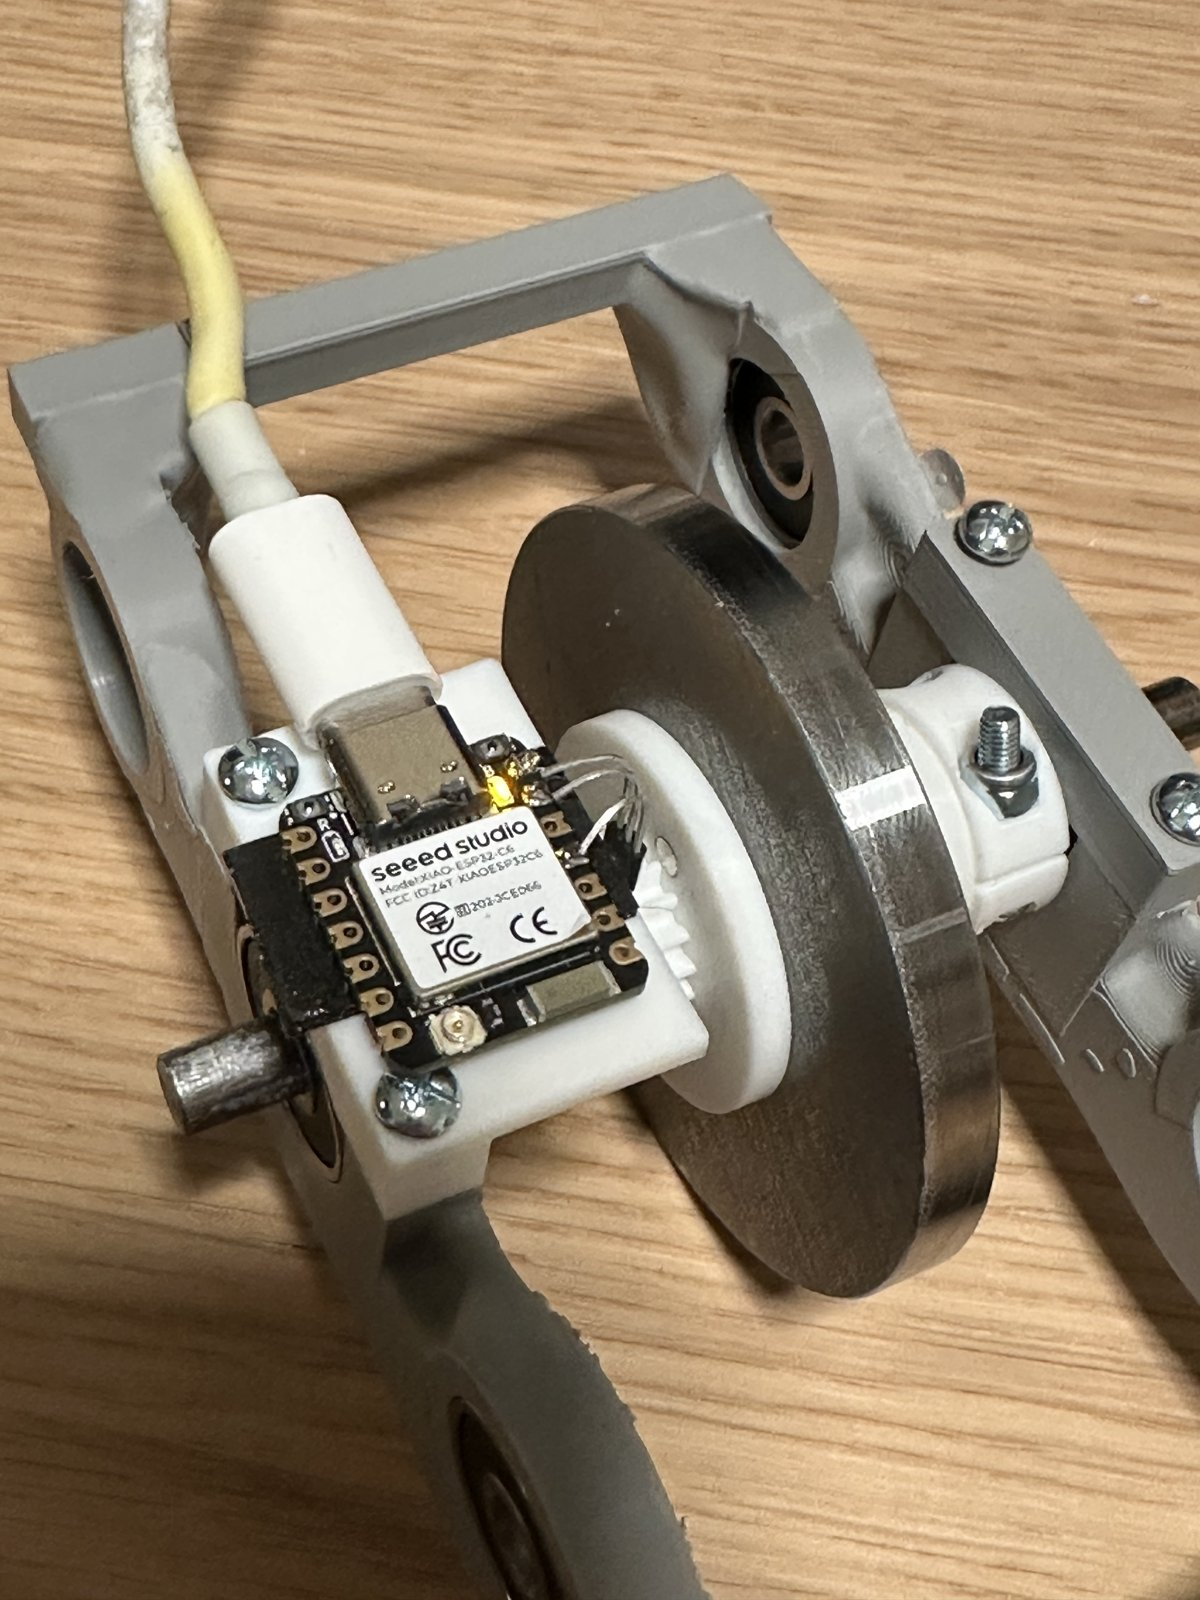
\includegraphics[width=0.42\textwidth]{Images/Foto/Ferdig/esp_oppsett.jpg}
    \caption[Måleoppsettet for utsnurring]{Måleoppsettet for utsnurring: ESP32 med Hall-sensor ved magnetskiva på svinghjulsakselen.}
    \label{fig:esp-oppsett}
\end{figure}

\paragraph{Lagrene på hjulakslene} er ikke målt hver for seg. De er av samme type som lagrene på svinghjulsakselen og regnes med samme tap per par, omregnet til en ekstra rullemotstand $T/r_h$.

\paragraph{Virkningsgraden i drivverket} er målt med utsnurring med bilen løftet, først med tannhjulet frakoblet og deretter koblet, med samme lagre og trommel. Med tannhjulet koblet snurrer også drivakselen med hjulene og det store tannhjulet, og treghetsmomentet øker med deres treghetsmoment delt på $i^2$, omtrent \SI{1,8}{\percent}. Forskjellen i tapsmoment ved samme turtall er tapet i drivverket redusert til svinghjulsakselen, $T_\text{dv}$. Det omfatter tannhjulsinngrepet, lagrene på drivakselen og luftmotstanden på hjulene.

Utsnurringen måler tapet uten last. Under kjøring overfører drivverket i tillegg momentet som holder bilen i gang, $T_\text{last} = C_{rr} m_b g r_h / i$ ved svinghjulsakselen. Den ekvivalente virkningsgraden ved kjøring er da
\begin{equation}
    \eta = \frac{T_\text{last}}{T_\text{last} + T_\text{dv}} .
    \label{eq:eta-drivverk}
\end{equation}
Det forutsetter at tapet i inngrepet øker lite med lasten, noe som er rimelig ved så små momenter.

\paragraph{Friksjon mot underlaget.} \textbf{PLASSHOLDER: beskriv målingen av rullemotstanden, for eksempel at bilen uten svinghjul trilles ned et skråplan eller slippes med kjent fart, og av friksjonen mellom dekk og underlag, for eksempel helningsvinkelen der bilen med låste hjul begynner å skli.}

\paragraph{Sluring ved nedsetting} er ikke målt direkte, men beregnet i simuleringen. Direkte måling krever en sensor på drivakselen og er utsatt til MAST2007.

\subsection{Kjøretest}
\label{sec:metode-kjoretest}
Kjøretestene gjøres med hele bilen på et parkett- eller laminatgulv (figur~\ref{fig:testoppsett}). Svinghjulet trekkes opp med snor på trommelen mens bilen holdes løftet, og bilen settes ned med svinghjulet i gang, slik konkurransereglene krever. Startlinja er startretningen forlenget. Lengden $L$ måles med målebånd som rett linje fra startpunktet til der bilen stopper, og sideavviket $y$ som den vinkelrette avstanden fra stoppunktet til startlinja, positivt mot høyre og negativt mot venstre (figur~\ref{fig:testoppsett}c). Alle forsøk registreres, også mislykkede.

\begin{figure}[H]
    \centering
    \begin{subfigure}[b]{0.36\textwidth}
        \centering
        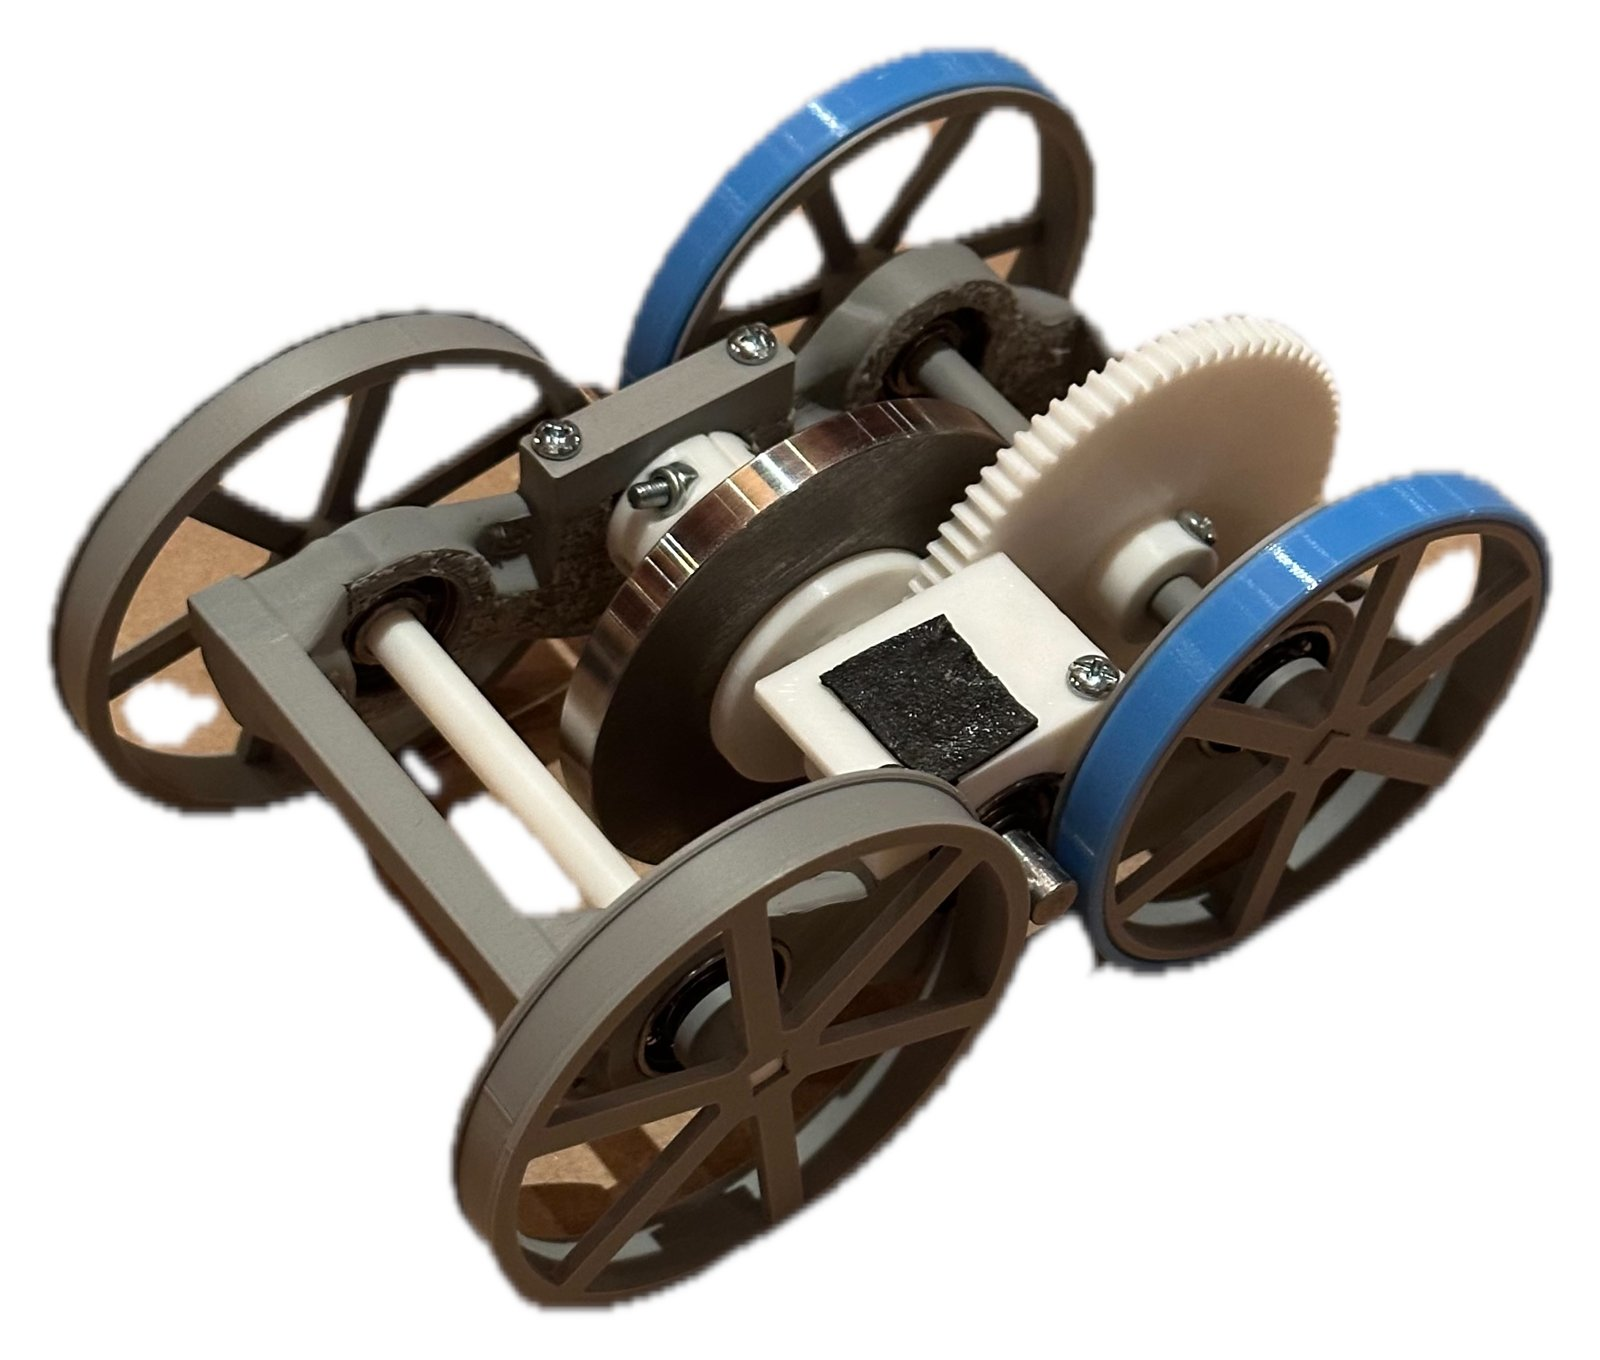
\includegraphics[width=\textwidth]{Images/Foto/Ferdig/bil_skraatt_bak.jpg}
        \caption{Bilen som testet}
    \end{subfigure}
    \hfill
    \begin{subfigure}[b]{0.27\textwidth}
        \centering
        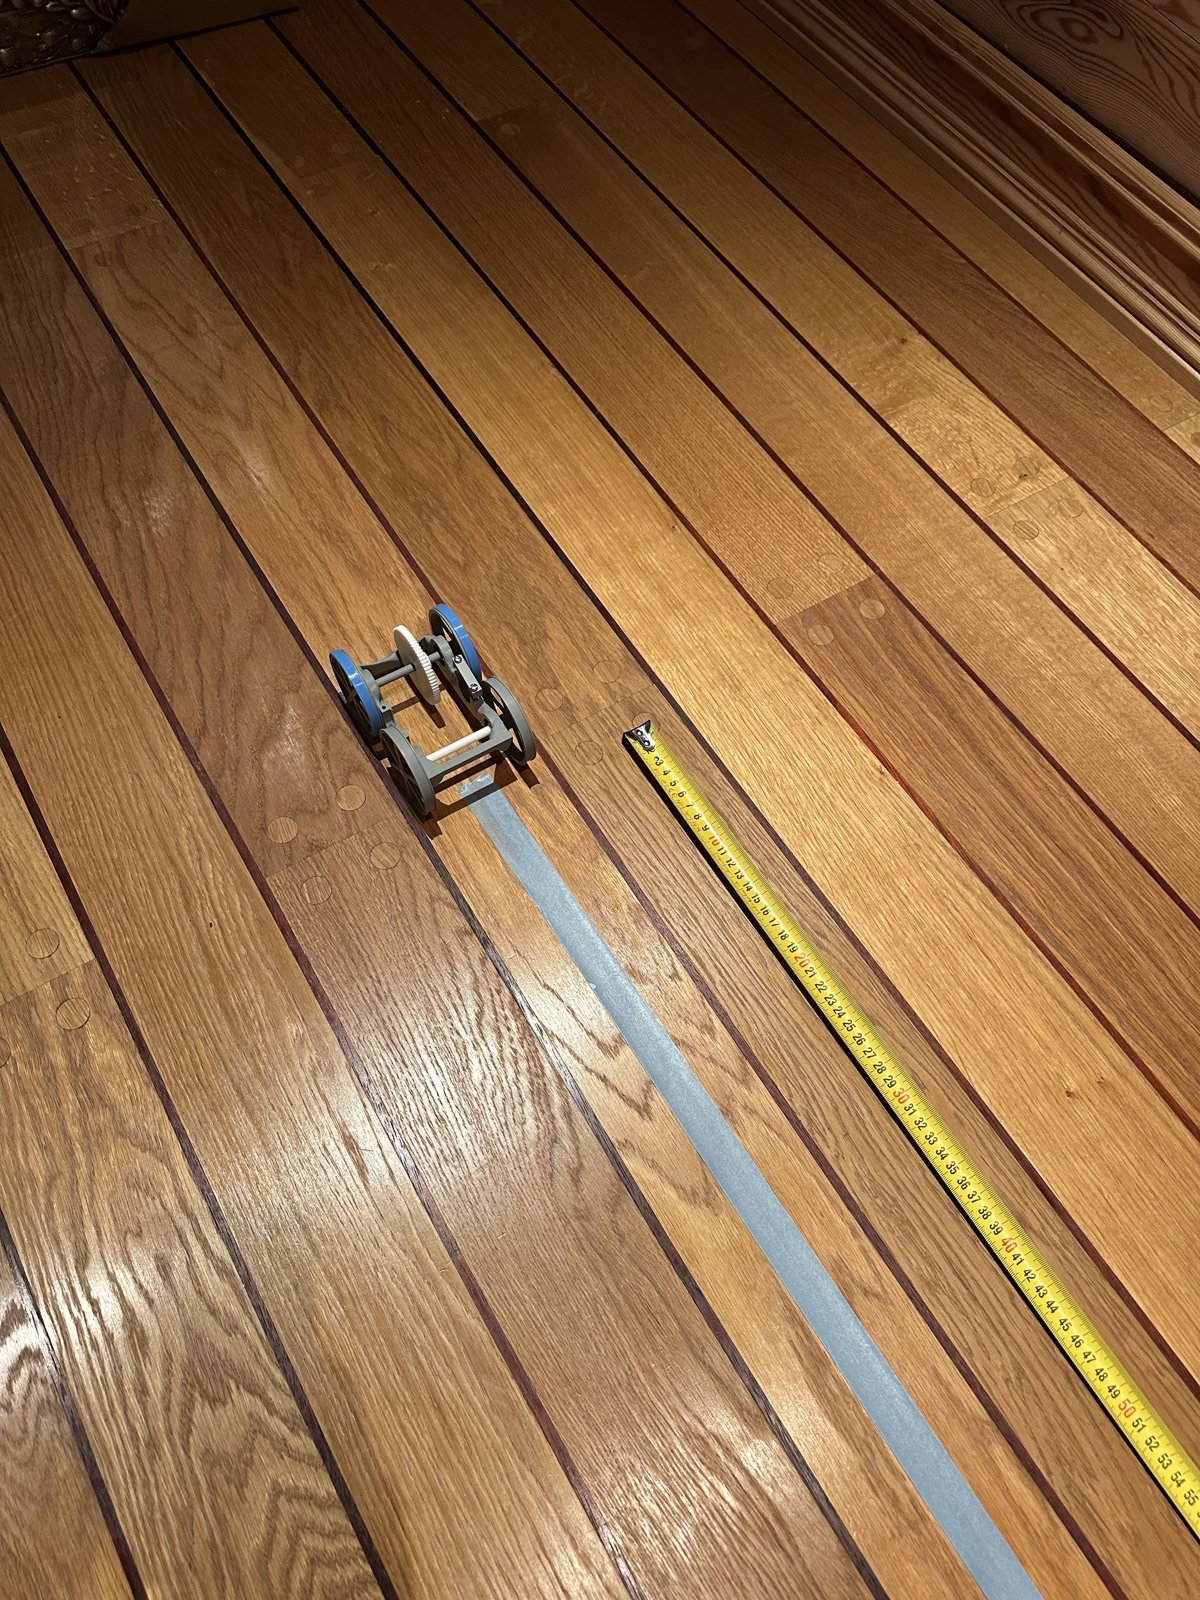
\includegraphics[width=\textwidth]{Images/Foto/Ferdig/testoppsett.jpg}
        \caption{Testoppsett}
    \end{subfigure}
    \hfill
    \begin{subfigure}[b]{0.25\textwidth}
        \centering
        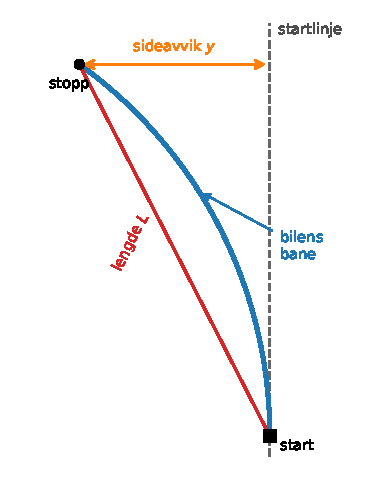
\includegraphics[width=\textwidth]{Images/Kjoretest/maalegeometri.pdf}
        \caption{Lengde og sideavvik}
    \end{subfigure}
    \caption[Kjøretesten]{Kjøretesten. (a) Bilen slik den ble kjøretestet, \SI{270}{g}. (b) Gulvet med målebånd. (c) Lengden måles som rett linje fra start til stopp, og sideavviket vinkelrett på startlinja. Banen er forsøk 4 i den første kjøretesten.}
    \label{fig:testoppsett}
\end{figure}

Hvis bilen kjører i en sirkelbue som starter langs startlinja, gir lengden $L$ og sideavviket $y$ svingradiusen
\begin{equation}
    R = \frac{L^2}{2\,|y|}.
    \label{eq:svingradius}
\end{equation}
Repeterbarheten (R4) vurderes med standardavviket av lengden i prosent av snittet, og retningsstabiliteten (R5) med snittet av $|y|/L$.

\begin{comment}
\subsection{Mål for testen}
Testene skal dokumentere funksjon, kjøredistanse, repeterbarhet og retningsstabilitet.

\subsection{Hypotese}
% Formuler hva testene forventes å vise, for eksempel forventet kjøredistanse ut fra overslaget i teorikapittelet.

\subsection{Testoppsett, utstyr og underlag}
Underlag, måleutstyr og måleoppløsning beskrives før gjennomføring.

\subsection{Standardisert opptrekk og startprosedyre}
Bilen holdes løftet under opptrekk og settes ned med svinghjulet i gang, i tråd med konkurransereglene. Trådlengde, opptrekksmåte, startposisjon, retning og frigjøring holdes så like som mulig. Lik trådlengde alene sikrer ikke lik tilført energi; variasjon i opptrekk registreres som en mulig feilkilde.

\subsection{Testdesign}
Planen er å gjennomføre 10--20 referansekjøringer og minst 10 kjøringer per sammenlignet konfigurasjon. Endre én faktor om gangen der dette er praktisk, og registrer prototypeversjon og testrekkefølge. Definer måling av kjøredistanse og sideavvik entydig før testene.

\subsection{Registrering og behandling av data}
Loggen skal inneholde kjøringsnummer, dato, konfigurasjon, opptrekk, distanse, sideavvik, vellykket eller mislykket kjøring og observasjoner. Alle forsøk registreres; eventuelle utelatelser begrunnes. Rapporter gjennomsnitt, standardavvik, antall forsøk og suksessandel med tydelig angivelse av hvilke forsøk som inngår.
% Gi formlene for gjennomsnitt og standardavvik som brukes i analysen.

\subsection{Måleusikkerhet og feilkilder}
% Vurder opptrekk, underlag, startretning, måleavlesning og endringer i prototypen mellom kjøringene.
\end{comment}
